% actor-constellation.tex
% Multi-actor constellation of a data centre assemblage (CAS diagram)
% Compile with: pdflatex --shell-escape actor-constellation.tex
\documentclass[tikz,border=5pt]{standalone}
\usepackage{tikz}
\usetikzlibrary{arrows.meta,positioning,shapes.geometric,fit,backgrounds}

%% ── Colour definitions ────────────────────────────────────────────────────────
\definecolor{dcblue}{RGB}{31,73,125}      % core operators
\definecolor{dcaccent}{RGB}{192,80,77}    % community layer
\definecolor{dcgray}{RGB}{89,89,89}       % governance / territorial layer
\definecolor{dcgold}{RGB}{155,118,29}     % financial layer
\definecolor{dcgreen}{RGB}{56,118,29}     % infrastructure layer
\definecolor{dclightbg}{RGB}{237,242,250} % background fill for core

%% ── Global style defaults ─────────────────────────────────────────────────────
\tikzset{
  %% node styles
  core/.style={
    draw=dcblue, fill=dclightbg, thick,
    rounded corners=4pt,
    font=\footnotesize\bfseries,
    text=dcblue,
    text width=3.0cm, align=center,
    minimum height=1.0cm,
  },
  actor/.style={
    draw=#1, fill=white, semithick,
    rounded corners=3pt,
    font=\footnotesize,
    text=#1,
    text width=2.6cm, align=center,
    minimum height=0.85cm,
  },
  actor/.default=dcgray,
  %% edge styles
  financial edge/.style={
    dashed, thick, color=dcgold,
    -{Stealth[length=5pt]},
  },
  governance edge/.style={
    solid, thick, color=dcgray,
    -{Stealth[length=5pt]},
  },
  community edge/.style={
    dotted, very thick, color=dcaccent,
    -{Stealth[length=5pt]},
  },
  infra edge/.style={
    double, double distance=1.2pt, thick, color=dcgreen,
    -{Stealth[length=5pt]},
  },
  %% legend entries
  legend box/.style={
    draw=dcgray!40, fill=white, rounded corners=2pt,
    inner sep=4pt,
  },
}

\begin{document}
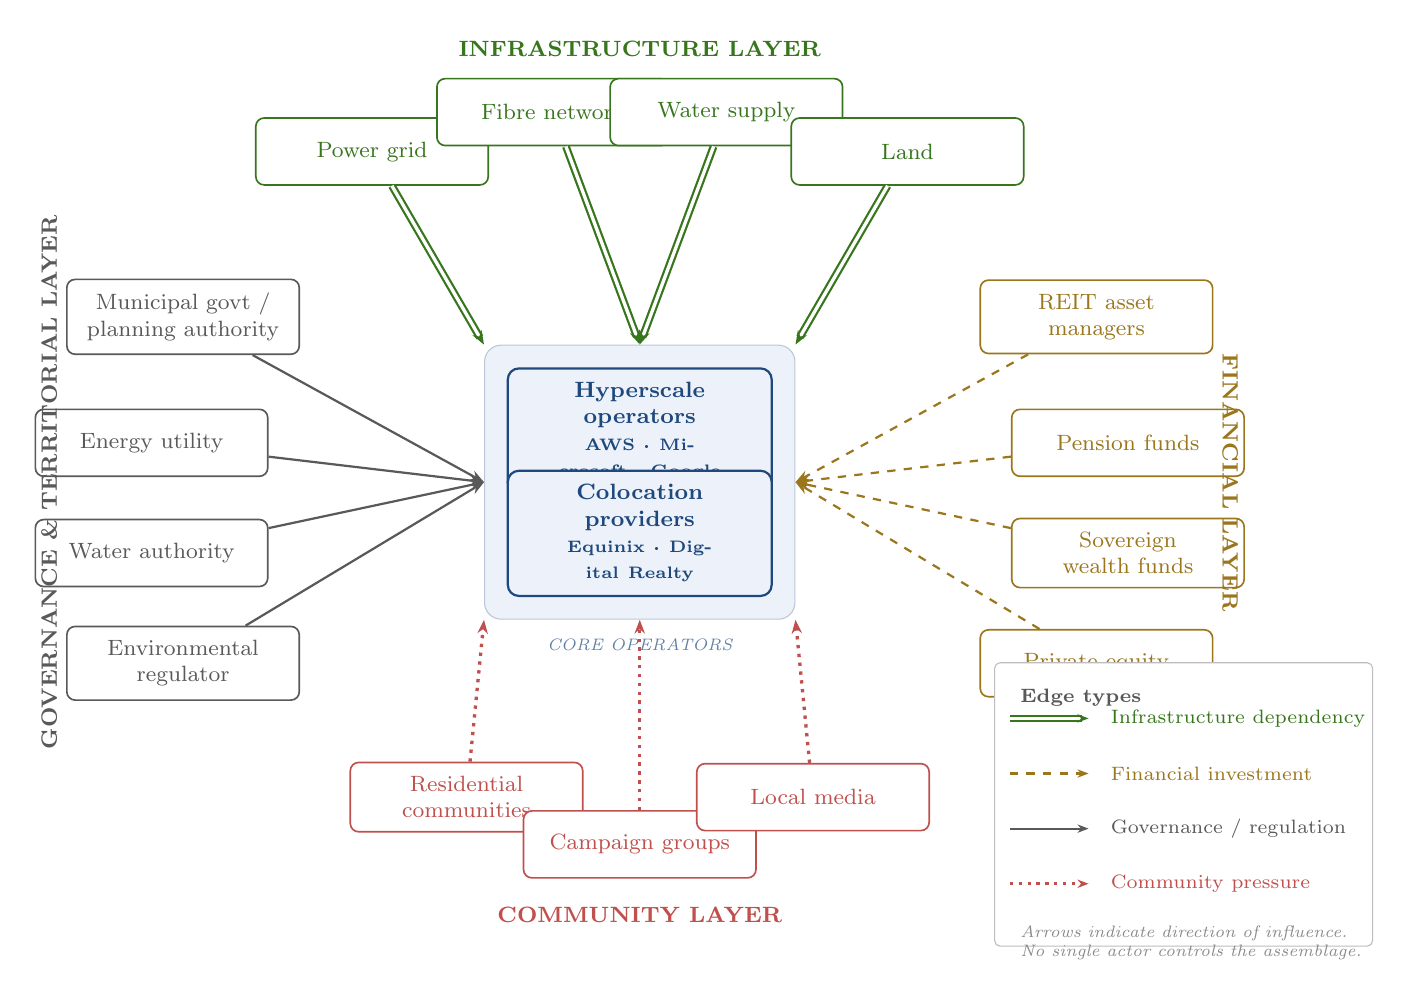
\begin{tikzpicture}[
    node distance = 0pt,
    every node/.append style={inner sep=5pt},
  ]

  %% ════════════════════════════════════════════════════════════════════════════
  %% CORE OPERATORS  (centre)
  %% ════════════════════════════════════════════════════════════════════════════
  \node[core] (hyper) at (0, 0.65)
    {Hyperscale operators\\{\fontsize{6}{7}\selectfont AWS · Microsoft · Google}};

  \node[core] (colo) at (0,-0.65)
    {Colocation providers\\{\fontsize{6}{7}\selectfont Equinix · Digital Realty}};

  %% light background behind the two core nodes
  \begin{scope}[on background layer]
    \node[draw=dcblue!30, fill=dclightbg, rounded corners=6pt,
          fit=(hyper)(colo), inner sep=8pt] (core box) {};
  \end{scope}

  \node[font=\fontsize{6}{7}\selectfont\itshape, text=dcblue!70,
        below=2pt of core box.south] {CORE OPERATORS};


  %% ════════════════════════════════════════════════════════════════════════════
  %% INFRASTRUCTURE LAYER  (top arc)
  %% ════════════════════════════════════════════════════════════════════════════
  \node[actor=dcgreen] (power)   at (-3.4, 4.2) {Power grid};
  \node[actor=dcgreen] (fibre)   at (-1.1, 4.7) {Fibre network};
  \node[actor=dcgreen] (water)   at ( 1.1, 4.7) {Water supply};
  \node[actor=dcgreen] (land)    at ( 3.4, 4.2) {Land};

  %% ════════════════════════════════════════════════════════════════════════════
  %% FINANCIAL LAYER  (right arc)
  %% ════════════════════════════════════════════════════════════════════════════
  \node[actor=dcgold] (reit)    at ( 5.8,  2.1) {REIT asset managers};
  \node[actor=dcgold] (pension) at ( 6.2,  0.5) {Pension funds};
  \node[actor=dcgold] (swf)     at ( 6.2, -0.9) {Sovereign wealth funds};
  \node[actor=dcgold] (pe)      at ( 5.8, -2.3) {Private equity};

  %% ════════════════════════════════════════════════════════════════════════════
  %% GOVERNANCE / TERRITORIAL LAYER  (left arc)
  %% ════════════════════════════════════════════════════════════════════════════
  \node[actor=dcgray] (muni)    at (-5.8,  2.1)
    {Municipal govt /\\planning authority};
  \node[actor=dcgray] (energy)  at (-6.2,  0.5) {Energy utility};
  \node[actor=dcgray] (waterau) at (-6.2, -0.9) {Water authority};
  \node[actor=dcgray] (envreg)  at (-5.8, -2.3) {Environmental regulator};

  %% ════════════════════════════════════════════════════════════════════════════
  %% COMMUNITY LAYER  (bottom arc)
  %% ════════════════════════════════════════════════════════════════════════════
  \node[actor=dcaccent] (residents) at (-2.2, -4.0) {Residential communities};
  \node[actor=dcaccent] (campaign)  at ( 0,   -4.6) {Campaign groups};
  \node[actor=dcaccent] (media)     at ( 2.2, -4.0) {Local media};


  %% ════════════════════════════════════════════════════════════════════════════
  %% EDGES — infrastructure (double green)
  %% ════════════════════════════════════════════════════════════════════════════
  \draw[infra edge] (power)   -- (core box.north west);
  \draw[infra edge] (fibre)   -- (core box.north);
  \draw[infra edge] (water)   -- (core box.north);
  \draw[infra edge] (land)    -- (core box.north east);

  %% EDGES — financial (dashed gold)
  \draw[financial edge] (reit)    -- (core box.east);
  \draw[financial edge] (pension) -- (core box.east);
  \draw[financial edge] (swf)     -- (core box.east);
  \draw[financial edge] (pe)      -- (core box.east);

  %% EDGES — governance (solid gray)
  \draw[governance edge] (muni)    -- (core box.west);
  \draw[governance edge] (energy)  -- (core box.west);
  \draw[governance edge] (waterau) -- (core box.west);
  \draw[governance edge] (envreg)  -- (core box.west);

  %% EDGES — community (dotted red)
  \draw[community edge] (residents) -- (core box.south west);
  \draw[community edge] (campaign)  -- (core box.south);
  \draw[community edge] (media)     -- (core box.south east);


  %% ════════════════════════════════════════════════════════════════════════════
  %% LAYER LABELS  (arc annotations)
  %% ════════════════════════════════════════════════════════════════════════════
  \node[font=\footnotesize\bfseries, text=dcgreen,  rotate=0 ] at (0,    5.5)
    {INFRASTRUCTURE LAYER};
  \node[font=\footnotesize\bfseries, text=dcgold,   rotate=-90] at (7.5,  0.0)
    {FINANCIAL LAYER};
  \node[font=\footnotesize\bfseries, text=dcgray,   rotate=90 ] at (-7.5, 0.0)
    {GOVERNANCE \& TERRITORIAL LAYER};
  \node[font=\footnotesize\bfseries, text=dcaccent, rotate=0 ] at (0,   -5.5)
    {COMMUNITY LAYER};


  %% ════════════════════════════════════════════════════════════════════════════
  %% LEGEND  (bottom-right corner)
  %% ════════════════════════════════════════════════════════════════════════════
  \begin{scope}[shift={(4.5,-5.9)}]
    \node[legend box, minimum width=4.8cm, minimum height=3.6cm,
          anchor=south west] (legbox) at (0,0) {};
    \node[font=\fontsize{7}{8}\selectfont\bfseries, anchor=north west,
          text=dcgray] at (0.15,3.45) {Edge types};

    %% infrastructure
    \draw[infra edge, -{Stealth[length=4pt]}]
      (0.2,2.9) -- (1.2,2.9);
    \node[font=\fontsize{7}{8}\selectfont, anchor=west, text=dcgreen]
      at (1.3,2.9) {Infrastructure dependency};

    %% financial
    \draw[financial edge, -{Stealth[length=4pt]}]
      (0.2,2.2) -- (1.2,2.2);
    \node[font=\fontsize{7}{8}\selectfont, anchor=west, text=dcgold]
      at (1.3,2.2) {Financial investment};

    %% governance
    \draw[governance edge, -{Stealth[length=4pt]}]
      (0.2,1.5) -- (1.2,1.5);
    \node[font=\fontsize{7}{8}\selectfont, anchor=west, text=dcgray]
      at (1.3,1.5) {Governance / regulation};

    %% community
    \draw[community edge, -{Stealth[length=4pt]}]
      (0.2,0.8) -- (1.2,0.8);
    \node[font=\fontsize{7}{8}\selectfont, anchor=west, text=dcaccent]
      at (1.3,0.8) {Community pressure};

    \node[font=\fontsize{6}{7}\selectfont\itshape, text=dcgray!70,
          anchor=north west, text width=4.4cm]
      at (0.15,0.45)
      {Arrows indicate direction of influence.\\
       No single actor controls the assemblage.};
  \end{scope}

\end{tikzpicture}
\end{document}
